\documentclass{article} % For LaTeX2e
\usepackage{iclr2021_conference,times}

% Optional math commands from https://github.com/goodfeli/dlbook_notation.
% DO NOT MODIFY THIS COMMENT
% read `https://github.com/James-Yu/LaTeX-Workshop/wiki/Compile#the-root-file`
% read `https://github.com/James-Yu/LaTeX-Workshop/issues/1165`
% !TEX root = iclr2021_conference.tex

%%%%% NEW MATH DEFINITIONS %%%%%

\usepackage{amsmath,amsfonts,bm}

% Mark sections of captions for referring to divisions of figures
\newcommand{\figleft}{{\em (Left)}}
\newcommand{\figcenter}{{\em (Center)}}
\newcommand{\figright}{{\em (Right)}}
\newcommand{\figtop}{{\em (Top)}}
\newcommand{\figbottom}{{\em (Bottom)}}
\newcommand{\captiona}{{\em (a)}}
\newcommand{\captionb}{{\em (b)}}
\newcommand{\captionc}{{\em (c)}}
\newcommand{\captiond}{{\em (d)}}

% Highlight a newly defined term
\newcommand{\newterm}[1]{{\bf #1}}


% Figure reference, lower-case.
\def\figref#1{figure~\ref{#1}}
% Figure reference, capital. For start of sentence
\def\Figref#1{Figure~\ref{#1}}
\def\twofigref#1#2{figures \ref{#1} and \ref{#2}}
\def\quadfigref#1#2#3#4{figures \ref{#1}, \ref{#2}, \ref{#3} and \ref{#4}}
% Section reference, lower-case.
\def\secref#1{section~\ref{#1}}
% Section reference, capital.
\def\Secref#1{Section~\ref{#1}}
% Reference to two sections.
\def\twosecrefs#1#2{sections \ref{#1} and \ref{#2}}
% Reference to three sections.
\def\secrefs#1#2#3{sections \ref{#1}, \ref{#2} and \ref{#3}}
% Reference to an equation, lower-case.
\def\eqref#1{equation~\ref{#1}}
% Reference to an equation, upper case
\def\Eqref#1{Equation~\ref{#1}}
% A raw reference to an equation---avoid using if possible
\def\plaineqref#1{\ref{#1}}
% Reference to a chapter, lower-case.
\def\chapref#1{chapter~\ref{#1}}
% Reference to an equation, upper case.
\def\Chapref#1{Chapter~\ref{#1}}
% Reference to a range of chapters
\def\rangechapref#1#2{chapters\ref{#1}--\ref{#2}}
% Reference to an algorithm, lower-case.
\def\algref#1{algorithm~\ref{#1}}
% Reference to an algorithm, upper case.
\def\Algref#1{Algorithm~\ref{#1}}
\def\twoalgref#1#2{algorithms \ref{#1} and \ref{#2}}
\def\Twoalgref#1#2{Algorithms \ref{#1} and \ref{#2}}
% Reference to a part, lower case
\def\partref#1{part~\ref{#1}}
% Reference to a part, upper case
\def\Partref#1{Part~\ref{#1}}
\def\twopartref#1#2{parts \ref{#1} and \ref{#2}}

\def\ceil#1{\lceil #1 \rceil}
\def\floor#1{\lfloor #1 \rfloor}
\def\1{\bm{1}}
\newcommand{\train}{\mathcal{D}}
\newcommand{\valid}{\mathcal{D_{\mathrm{valid}}}}
\newcommand{\test}{\mathcal{D_{\mathrm{test}}}}

\def\eps{{\epsilon}}


% Random variables
\def\reta{{\textnormal{$\eta$}}}
\def\ra{{\textnormal{a}}}
\def\rb{{\textnormal{b}}}
\def\rc{{\textnormal{c}}}
\def\rd{{\textnormal{d}}}
\def\re{{\textnormal{e}}}
\def\rf{{\textnormal{f}}}
\def\rg{{\textnormal{g}}}
\def\rh{{\textnormal{h}}}
\def\ri{{\textnormal{i}}}
\def\rj{{\textnormal{j}}}
\def\rk{{\textnormal{k}}}
\def\rl{{\textnormal{l}}}
% rm is already a command, just don't name any random variables m
\def\rn{{\textnormal{n}}}
\def\ro{{\textnormal{o}}}
\def\rp{{\textnormal{p}}}
\def\rq{{\textnormal{q}}}
\def\rr{{\textnormal{r}}}
\def\rs{{\textnormal{s}}}
\def\rt{{\textnormal{t}}}
\def\ru{{\textnormal{u}}}
\def\rv{{\textnormal{v}}}
\def\rw{{\textnormal{w}}}
\def\rx{{\textnormal{x}}}
\def\ry{{\textnormal{y}}}
\def\rz{{\textnormal{z}}}

% Random vectors
\def\rvepsilon{{\mathbf{\epsilon}}}
\def\rvtheta{{\mathbf{\theta}}}
\def\rva{{\mathbf{a}}}
\def\rvb{{\mathbf{b}}}
\def\rvc{{\mathbf{c}}}
\def\rvd{{\mathbf{d}}}
\def\rve{{\mathbf{e}}}
\def\rvf{{\mathbf{f}}}
\def\rvg{{\mathbf{g}}}
\def\rvh{{\mathbf{h}}}
\def\rvu{{\mathbf{i}}}
\def\rvj{{\mathbf{j}}}
\def\rvk{{\mathbf{k}}}
\def\rvl{{\mathbf{l}}}
\def\rvm{{\mathbf{m}}}
\def\rvn{{\mathbf{n}}}
\def\rvo{{\mathbf{o}}}
\def\rvp{{\mathbf{p}}}
\def\rvq{{\mathbf{q}}}
\def\rvr{{\mathbf{r}}}
\def\rvs{{\mathbf{s}}}
\def\rvt{{\mathbf{t}}}
\def\rvu{{\mathbf{u}}}
\def\rvv{{\mathbf{v}}}
\def\rvw{{\mathbf{w}}}
\def\rvx{{\mathbf{x}}}
\def\rvy{{\mathbf{y}}}
\def\rvz{{\mathbf{z}}}

% Elements of random vectors
\def\erva{{\textnormal{a}}}
\def\ervb{{\textnormal{b}}}
\def\ervc{{\textnormal{c}}}
\def\ervd{{\textnormal{d}}}
\def\erve{{\textnormal{e}}}
\def\ervf{{\textnormal{f}}}
\def\ervg{{\textnormal{g}}}
\def\ervh{{\textnormal{h}}}
\def\ervi{{\textnormal{i}}}
\def\ervj{{\textnormal{j}}}
\def\ervk{{\textnormal{k}}}
\def\ervl{{\textnormal{l}}}
\def\ervm{{\textnormal{m}}}
\def\ervn{{\textnormal{n}}}
\def\ervo{{\textnormal{o}}}
\def\ervp{{\textnormal{p}}}
\def\ervq{{\textnormal{q}}}
\def\ervr{{\textnormal{r}}}
\def\ervs{{\textnormal{s}}}
\def\ervt{{\textnormal{t}}}
\def\ervu{{\textnormal{u}}}
\def\ervv{{\textnormal{v}}}
\def\ervw{{\textnormal{w}}}
\def\ervx{{\textnormal{x}}}
\def\ervy{{\textnormal{y}}}
\def\ervz{{\textnormal{z}}}

% Random matrices
\def\rmA{{\mathbf{A}}}
\def\rmB{{\mathbf{B}}}
\def\rmC{{\mathbf{C}}}
\def\rmD{{\mathbf{D}}}
\def\rmE{{\mathbf{E}}}
\def\rmF{{\mathbf{F}}}
\def\rmG{{\mathbf{G}}}
\def\rmH{{\mathbf{H}}}
\def\rmI{{\mathbf{I}}}
\def\rmJ{{\mathbf{J}}}
\def\rmK{{\mathbf{K}}}
\def\rmL{{\mathbf{L}}}
\def\rmM{{\mathbf{M}}}
\def\rmN{{\mathbf{N}}}
\def\rmO{{\mathbf{O}}}
\def\rmP{{\mathbf{P}}}
\def\rmQ{{\mathbf{Q}}}
\def\rmR{{\mathbf{R}}}
\def\rmS{{\mathbf{S}}}
\def\rmT{{\mathbf{T}}}
\def\rmU{{\mathbf{U}}}
\def\rmV{{\mathbf{V}}}
\def\rmW{{\mathbf{W}}}
\def\rmX{{\mathbf{X}}}
\def\rmY{{\mathbf{Y}}}
\def\rmZ{{\mathbf{Z}}}

% Elements of random matrices
\def\ermA{{\textnormal{A}}}
\def\ermB{{\textnormal{B}}}
\def\ermC{{\textnormal{C}}}
\def\ermD{{\textnormal{D}}}
\def\ermE{{\textnormal{E}}}
\def\ermF{{\textnormal{F}}}
\def\ermG{{\textnormal{G}}}
\def\ermH{{\textnormal{H}}}
\def\ermI{{\textnormal{I}}}
\def\ermJ{{\textnormal{J}}}
\def\ermK{{\textnormal{K}}}
\def\ermL{{\textnormal{L}}}
\def\ermM{{\textnormal{M}}}
\def\ermN{{\textnormal{N}}}
\def\ermO{{\textnormal{O}}}
\def\ermP{{\textnormal{P}}}
\def\ermQ{{\textnormal{Q}}}
\def\ermR{{\textnormal{R}}}
\def\ermS{{\textnormal{S}}}
\def\ermT{{\textnormal{T}}}
\def\ermU{{\textnormal{U}}}
\def\ermV{{\textnormal{V}}}
\def\ermW{{\textnormal{W}}}
\def\ermX{{\textnormal{X}}}
\def\ermY{{\textnormal{Y}}}
\def\ermZ{{\textnormal{Z}}}

% Vectors
\def\vzero{{\bm{0}}}
\def\vone{{\bm{1}}}
\def\vmu{{\bm{\mu}}}
\def\vtheta{{\bm{\theta}}}
\def\va{{\bm{a}}}
\def\vb{{\bm{b}}}
\def\vc{{\bm{c}}}
\def\vd{{\bm{d}}}
\def\ve{{\bm{e}}}
\def\vf{{\bm{f}}}
\def\vg{{\bm{g}}}
\def\vh{{\bm{h}}}
\def\vi{{\bm{i}}}
\def\vj{{\bm{j}}}
\def\vk{{\bm{k}}}
\def\vl{{\bm{l}}}
\def\vm{{\bm{m}}}
\def\vn{{\bm{n}}}
\def\vo{{\bm{o}}}
\def\vp{{\bm{p}}}
\def\vq{{\bm{q}}}
\def\vr{{\bm{r}}}
\def\vs{{\bm{s}}}
\def\vt{{\bm{t}}}
\def\vu{{\bm{u}}}
\def\vv{{\bm{v}}}
\def\vw{{\bm{w}}}
\def\vx{{\bm{x}}}
\def\vy{{\bm{y}}}
\def\vz{{\bm{z}}}

% Elements of vectors
\def\evalpha{{\alpha}}
\def\evbeta{{\beta}}
\def\evepsilon{{\epsilon}}
\def\evlambda{{\lambda}}
\def\evomega{{\omega}}
\def\evmu{{\mu}}
\def\evpsi{{\psi}}
\def\evsigma{{\sigma}}
\def\evtheta{{\theta}}
\def\eva{{a}}
\def\evb{{b}}
\def\evc{{c}}
\def\evd{{d}}
\def\eve{{e}}
\def\evf{{f}}
\def\evg{{g}}
\def\evh{{h}}
\def\evi{{i}}
\def\evj{{j}}
\def\evk{{k}}
\def\evl{{l}}
\def\evm{{m}}
\def\evn{{n}}
\def\evo{{o}}
\def\evp{{p}}
\def\evq{{q}}
\def\evr{{r}}
\def\evs{{s}}
\def\evt{{t}}
\def\evu{{u}}
\def\evv{{v}}
\def\evw{{w}}
\def\evx{{x}}
\def\evy{{y}}
\def\evz{{z}}

% Matrix
\def\mA{{\bm{A}}}
\def\mB{{\bm{B}}}
\def\mC{{\bm{C}}}
\def\mD{{\bm{D}}}
\def\mE{{\bm{E}}}
\def\mF{{\bm{F}}}
\def\mG{{\bm{G}}}
\def\mH{{\bm{H}}}
\def\mI{{\bm{I}}}
\def\mJ{{\bm{J}}}
\def\mK{{\bm{K}}}
\def\mL{{\bm{L}}}
\def\mM{{\bm{M}}}
\def\mN{{\bm{N}}}
\def\mO{{\bm{O}}}
\def\mP{{\bm{P}}}
\def\mQ{{\bm{Q}}}
\def\mR{{\bm{R}}}
\def\mS{{\bm{S}}}
\def\mT{{\bm{T}}}
\def\mU{{\bm{U}}}
\def\mV{{\bm{V}}}
\def\mW{{\bm{W}}}
\def\mX{{\bm{X}}}
\def\mY{{\bm{Y}}}
\def\mZ{{\bm{Z}}}
\def\mBeta{{\bm{\beta}}}
\def\mPhi{{\bm{\Phi}}}
\def\mLambda{{\bm{\Lambda}}}
\def\mSigma{{\bm{\Sigma}}}

% Tensor
\DeclareMathAlphabet{\mathsfit}{\encodingdefault}{\sfdefault}{m}{sl}
\SetMathAlphabet{\mathsfit}{bold}{\encodingdefault}{\sfdefault}{bx}{n}
\newcommand{\tens}[1]{\bm{\mathsfit{#1}}}
\def\tA{{\tens{A}}}
\def\tB{{\tens{B}}}
\def\tC{{\tens{C}}}
\def\tD{{\tens{D}}}
\def\tE{{\tens{E}}}
\def\tF{{\tens{F}}}
\def\tG{{\tens{G}}}
\def\tH{{\tens{H}}}
\def\tI{{\tens{I}}}
\def\tJ{{\tens{J}}}
\def\tK{{\tens{K}}}
\def\tL{{\tens{L}}}
\def\tM{{\tens{M}}}
\def\tN{{\tens{N}}}
\def\tO{{\tens{O}}}
\def\tP{{\tens{P}}}
\def\tQ{{\tens{Q}}}
\def\tR{{\tens{R}}}
\def\tS{{\tens{S}}}
\def\tT{{\tens{T}}}
\def\tU{{\tens{U}}}
\def\tV{{\tens{V}}}
\def\tW{{\tens{W}}}
\def\tX{{\tens{X}}}
\def\tY{{\tens{Y}}}
\def\tZ{{\tens{Z}}}


% Graph
\def\gA{{\mathcal{A}}}
\def\gB{{\mathcal{B}}}
\def\gC{{\mathcal{C}}}
\def\gD{{\mathcal{D}}}
\def\gE{{\mathcal{E}}}
\def\gF{{\mathcal{F}}}
\def\gG{{\mathcal{G}}}
\def\gH{{\mathcal{H}}}
\def\gI{{\mathcal{I}}}
\def\gJ{{\mathcal{J}}}
\def\gK{{\mathcal{K}}}
\def\gL{{\mathcal{L}}}
\def\gM{{\mathcal{M}}}
\def\gN{{\mathcal{N}}}
\def\gO{{\mathcal{O}}}
\def\gP{{\mathcal{P}}}
\def\gQ{{\mathcal{Q}}}
\def\gR{{\mathcal{R}}}
\def\gS{{\mathcal{S}}}
\def\gT{{\mathcal{T}}}
\def\gU{{\mathcal{U}}}
\def\gV{{\mathcal{V}}}
\def\gW{{\mathcal{W}}}
\def\gX{{\mathcal{X}}}
\def\gY{{\mathcal{Y}}}
\def\gZ{{\mathcal{Z}}}

% Sets
\def\sA{{\mathbb{A}}}
\def\sB{{\mathbb{B}}}
\def\sC{{\mathbb{C}}}
\def\sD{{\mathbb{D}}}
% Don't use a set called E, because this would be the same as our symbol
% for expectation.
\def\sF{{\mathbb{F}}}
\def\sG{{\mathbb{G}}}
\def\sH{{\mathbb{H}}}
\def\sI{{\mathbb{I}}}
\def\sJ{{\mathbb{J}}}
\def\sK{{\mathbb{K}}}
\def\sL{{\mathbb{L}}}
\def\sM{{\mathbb{M}}}
\def\sN{{\mathbb{N}}}
\def\sO{{\mathbb{O}}}
\def\sP{{\mathbb{P}}}
\def\sQ{{\mathbb{Q}}}
\def\sR{{\mathbb{R}}}
\def\sS{{\mathbb{S}}}
\def\sT{{\mathbb{T}}}
\def\sU{{\mathbb{U}}}
\def\sV{{\mathbb{V}}}
\def\sW{{\mathbb{W}}}
\def\sX{{\mathbb{X}}}
\def\sY{{\mathbb{Y}}}
\def\sZ{{\mathbb{Z}}}

% Entries of a matrix
\def\emLambda{{\Lambda}}
\def\emA{{A}}
\def\emB{{B}}
\def\emC{{C}}
\def\emD{{D}}
\def\emE{{E}}
\def\emF{{F}}
\def\emG{{G}}
\def\emH{{H}}
\def\emI{{I}}
\def\emJ{{J}}
\def\emK{{K}}
\def\emL{{L}}
\def\emM{{M}}
\def\emN{{N}}
\def\emO{{O}}
\def\emP{{P}}
\def\emQ{{Q}}
\def\emR{{R}}
\def\emS{{S}}
\def\emT{{T}}
\def\emU{{U}}
\def\emV{{V}}
\def\emW{{W}}
\def\emX{{X}}
\def\emY{{Y}}
\def\emZ{{Z}}
\def\emSigma{{\Sigma}}

% entries of a tensor
% Same font as tensor, without \bm wrapper
\newcommand{\etens}[1]{\mathsfit{#1}}
\def\etLambda{{\etens{\Lambda}}}
\def\etA{{\etens{A}}}
\def\etB{{\etens{B}}}
\def\etC{{\etens{C}}}
\def\etD{{\etens{D}}}
\def\etE{{\etens{E}}}
\def\etF{{\etens{F}}}
\def\etG{{\etens{G}}}
\def\etH{{\etens{H}}}
\def\etI{{\etens{I}}}
\def\etJ{{\etens{J}}}
\def\etK{{\etens{K}}}
\def\etL{{\etens{L}}}
\def\etM{{\etens{M}}}
\def\etN{{\etens{N}}}
\def\etO{{\etens{O}}}
\def\etP{{\etens{P}}}
\def\etQ{{\etens{Q}}}
\def\etR{{\etens{R}}}
\def\etS{{\etens{S}}}
\def\etT{{\etens{T}}}
\def\etU{{\etens{U}}}
\def\etV{{\etens{V}}}
\def\etW{{\etens{W}}}
\def\etX{{\etens{X}}}
\def\etY{{\etens{Y}}}
\def\etZ{{\etens{Z}}}

% The true underlying data generating distribution
\newcommand{\pdata}{p_{\rm{data}}}
% The empirical distribution defined by the training set
\newcommand{\ptrain}{\hat{p}_{\rm{data}}}
\newcommand{\Ptrain}{\hat{P}_{\rm{data}}}
% The model distribution
\newcommand{\pmodel}{p_{\rm{model}}}
\newcommand{\Pmodel}{P_{\rm{model}}}
\newcommand{\ptildemodel}{\tilde{p}_{\rm{model}}}
% Stochastic autoencoder distributions
\newcommand{\pencode}{p_{\rm{encoder}}}
\newcommand{\pdecode}{p_{\rm{decoder}}}
\newcommand{\precons}{p_{\rm{reconstruct}}}

\newcommand{\laplace}{\mathrm{Laplace}} % Laplace distribution

\newcommand{\E}{\mathbb{E}}
\newcommand{\Ls}{\mathcal{L}}
\newcommand{\R}{\mathbb{R}}
\newcommand{\emp}{\tilde{p}}
\newcommand{\lr}{\alpha}
\newcommand{\reg}{\lambda}
\newcommand{\rect}{\mathrm{rectifier}}
\newcommand{\softmax}{\mathrm{softmax}}
\newcommand{\sigmoid}{\sigma}
\newcommand{\softplus}{\zeta}
\newcommand{\KL}{D_{\mathrm{KL}}}
\newcommand{\Var}{\mathrm{Var}}
\newcommand{\standarderror}{\mathrm{SE}}
\newcommand{\Cov}{\mathrm{Cov}}
% Wolfram Mathworld says $L^2$ is for function spaces and $\ell^2$ is for vectors
% But then they seem to use $L^2$ for vectors throughout the site, and so does
% wikipedia.
\newcommand{\normlzero}{L^0}
\newcommand{\normlone}{L^1}
\newcommand{\normltwo}{L^2}
\newcommand{\normlp}{L^p}
\newcommand{\normmax}{L^\infty}

\newcommand{\parents}{Pa} % See usage in notation.tex. Chosen to match Daphne's book.

\DeclareMathOperator*{\argmax}{arg\,max}
\DeclareMathOperator*{\argmin}{arg\,min}

\DeclareMathOperator{\sign}{sign}
\DeclareMathOperator{\Tr}{Tr}
\let\ab\allowbreak


\usepackage{hyperref}
\usepackage{url}
\usepackage{caption}

% I got these from this guide:
% https://shantoroy.com/latex/how-to-write-algorithm-in-latex/
% Which I use to highlight how we do the experiment.
\usepackage{algorithm}
\usepackage{arevmath}
\usepackage[noend]{algpseudocode}

\usepackage{graphicx}
\graphicspath{ {.} }

\setcitestyle{square,comma}


\title{Exploring Neural Network Modularity \\ Using Model Stitching}

% Authors must not appear in the submitted version, you uncomment a line below
% which is labeled "iclrfinalcopy" to anonymize or not.
\author{Adriano Hernandez, Rumen Dangovski \& Peter Y. Lu \thanks{You can find our other work at \url{http://www.a14z.blog/}, \url{http://super-ms.mit.edu/rumen.html}, and \url{https://peterparity.github.io/} respectively.} \\
MIT EECS\\
Cambridge, MA 02139, USA \\
\texttt{\{adrianoh,rumenrd,lup\}@mit.edu}
}

% The \author macro works with any number of authors. There are two commands
% used to separate the names and addresses of multiple authors: \And and \AND.
%
% Using \And between authors leaves it to \LaTeX{} to determine where to break
% the lines. Using \AND forces a linebreak at that point. So, if \LaTeX{}
% puts 3 of 4 authors names on the first line, and the last on the second
% line, try using \AND instead of \And before the third author name.

\newcommand{\fix}{\marginpar{FIX}}
\newcommand{\new}{\marginpar{NEW}}

\iclrfinalcopy % Uncomment for camera-ready version, but NOT for submission.
\begin{document}

\maketitle

\begin{abstract}
We expand \textit{model stitching} (Lenc \& Vedaldi 2015) as a methodology to compare neural networks.
Previously, Bansal, Nakkiran \& Barak used it to compare the representations learned by differently seeded
and/or trained neural networks.
We use it to compare the representations learned by neural networks with different architectures.
This enables us to reveal interesting behavior of model stitching. Namely, we find that stitching, 
based on convolutions, for small ResNets, can reach unexpectedly
high accuracy for intuitively different layers if those layers come earlier in the first (sender) network than in
the second (receiver). This leads us to hypothesize that stitches are not in fact learning to match the
representations expected by receiver layers, but instead to find different representations which nonetheless
yield similar results.
We do a simple numerical analysis to test this hypothesis and it yields mixed results.
\end{abstract}

\section{Introduction}
\label{Introduction}
The success of deep learning for visual recognition has been attributed to the ability of neural networks to learn
good representations of their training data \cite{Rumelhart1986LearningIR}. That is, intermediate outputs (which we refer
to as ``representations'') of good neural networks 
are believed to encode meaningful information about their inputs, which these neural networks use for classification and/or other
downstream machine learning tasks \cite{goodfellow2016deep}.
However, our understanding of these representations is somewhat limited. Though
deep learning interpretability research, particularly for computer vision, has helped us
to intuitively grasp what deep neural 
networks are learning, we do not
know why good representations are learned, nor do we have a robust theory to characterize them. For example, we do not
know how to compare representations effectively.

Being unable to compare representations is a fundamental limitation because it precludes us from understanding whether
different models are learning essentially the same thing. This is important, because one of the great hopes of the authors
of this paper is that
different neural networks are able to learn, by some measure, qualitatively similar representations, even if they are
numerically, or superficially, different. Metaphorically,
we would like to find that models learn ``the same sentences in different languages.''

Since two different representations can encode the same underlying information differently, one of the goals of this
paper is to advance our ability to ``translate these different languages,'' so to speak. Armed with such an ability,
if we found that indeed, most neural networks for certain
common tasks learn to encode the same
underlying information in their representations, that fact would lend credence to the belief that deep neural
networks, can learn meaningful concepts (if we can call representations ``concepts'')
like a human, since it is an unlikely coincidence that so many
different learners converge to similar representations.

At the very least this would be of philosophical interest and encourage explanatory theoretical research.
However, the ability to compare representations could empower us in more practical ways as well.
For example, we could use representational comparisons
to more rigorously test novel architectures based on older well-known ones. More generally, we could
use our existing knowledge about specific deep neural networks to gain more knowledge about others, quickly.
Thus, we want to be able to compare neural network representations.

\subsection*{Organization}
We first discuss related work in \hyperref[RelatedWork]{Section 2}. Subsequently we will provide a high-level view of our
contribution in \hyperref[Contribution]{Section 3} and explain our method of stitching in \hyperref[Stitching]{Section 4}.
In \hyperref[ExperimentalSetup]{Section 5} and \hyperref[Results]{Section 6} we will discuss our experimental setup and
results respectively, after which we wrap up with a conclusion in \hyperref[Conclusion]{Section 7}. Tables for one of
our numerical tests are available in the \hyperref[Appendix]{Appendix}.

\section{Related Work}
\label{RelatedWork}
Many non-learned similarity measures exist such as Centered Kernel Alignment \cite{Kornblith2019SimilarityON} and
Canonical Correlation Analysis \cite{Morcos2018InsightsOR}.

These may or may not be useful to explore the similarity of different representations. However, their efficacy relies
on the ingenuity of their designers since these measures are rather ad-hoc \cite{Bansal2021RevisitingMS}.
Recent research \cite{Ding2021GroundingRS} argues that some supposed improvements in these measures do not generalize.
Thus, we decide not to use these measures because results which use them their use are difficult to gague.
Instead, we choose a measure that depends entirely on accuracy: model stitching.

\section{Our Contribution}
\label{Contribution}
Recent advances in model stitching \cite{Bansal2021RevisitingMS} have made great strides towards the goal of effectively
comparing representations. Bansal et al. elaborate and use model stitching to confirm that architecturally similar
neural networks learn similar representations for computer vision.

They give us tantalizing results with positive practical by-products\footnote{
   They confirm that, on standard datasets, such as CIFAR-10, standard ResNets, such as ResNet18, are able to learn similar
   representations irrespective of their initial random seeds, layer widths, or (to a limited extent) training methodology.
   They use this finding to show that stitching wider neural networks into more narrow ones can improve performance. Moreover,
   they use stitching to tell how fast different layers converge to good solutions, which enables them to freeze
   fast-converging layers during training to save compute.
}.
In doing so open up a space of possibility for future research, and we see two main directions to explore.

\textbf{Different Architectures and Layer Shapes.} Bansal et al. only confirm that networks with the same 
fundamental architecture have similar representations at
the exact same layers. It is trickier to compare the representations of neural networks with different architectures
since they have different shapes, but in some respects this is the more meaningful and interesting thing to do.

\textbf{Sanity Testing Stitching.} Bansal et al. ignore a subtle point regarding the ability 
of stitching to compare representations. Model stitching essentially checks whether two representations
are interchangeable with minor modifications, using a \textit{learned} transformation to learn the best
such ``modifications.'' However, the transformation, which we call the stitch, is trained using backpropagation
from a downstream task like classification. It may not be necessary that two representations be ``similar,'' either
numerically or intuitively, for the stitched model to reach high task accuracy.

Our paper seeks to tackle these two questions. Firstly, we extend stitching in a simple way to be able to compare
different layers of off-the-shelf computer vision models. Secondly, we analyse 
whether different neural networks learning similar
representations. Lastly, we analyse whether stitching is a good metric in these cases using a simple numerical test. We
find that our simple extension of stitching yields unexpectedly high similarity for layers we thought should be different.
This result holds true, empirically, for all small simple ResNets \cite{He2016DeepRL} on CIFAR-10 \cite{CIFAR10},
varied by their random seed. This motivates
us to understand whether our stitches are actually behaving in the way we expect numerically. Our numerical test is not
fully conclusive, but suggests that not all stitches behave as expected.

\section{Stitching}
\label{Stitching}
We broaden the definition of stitching very little from that as defined in \cite{Bansal2021RevisitingMS}. In that paper,
stitching involved taking the intermediate output of some layer, which we call the sender, transforming it, and then
inputting that into an intermediate input in another network. We call the layer we input into the receiver. We
will also refer to the two networks, respectively, as sender and receiver when convenient and contextually clear.
The representation that would normally be recieved by the receiver we call the expected representation
\footnote{The expected representation is sent by
the expected sender: the previous layer in the receiver network.}.

The layers up to the sender (inclusive) we call a prefix and the layers from the receiver to the end (inclusive) we call
a suffix. The transformation used is called the stitch, and it is learned\footnote{We use gradient descent for simplicity.}
on a frozen\footnote{``Frozen'' refers to the fact that the weights are not updated during the backwards pass.}
prefix/suffix pair. The network formed by concatenating the sender prefix, the stitch, and the receiver
suffix, is called the stitched network, portrayed in \hyperref[Figure1]{Figure 1}. Just like Bansal et al., we use the task accuracy of the stitched network as our
primary training task.

The stitch belongs to a simple function class such as 1x1 convolutions (depthwise) or
a linear layer. Bansal et al. pick these function classes since, if the sender and receiver networks are in the same
function class, the stitched network will also be in that same function class. However, since for us the sender and
receiver networks are not in the same function class, we allow stitches that modify the function class in minor ways.
We expand the class of stitches to include strided convolutions
\footnote{Our convolutions have stride equal to kernel width, so as to downsample
by some constant factor.} as well as 1x1 convolutions of nearest-upsampled layers
\footnote{Nearest-upsampled means that each pixel
is copied a constant number of times, corresponding to a square grid of identical pixels}.

\label{Figure1}
\begin{center}
   \begin{figure}[h!]
      \centering
      \caption{Stitching}
      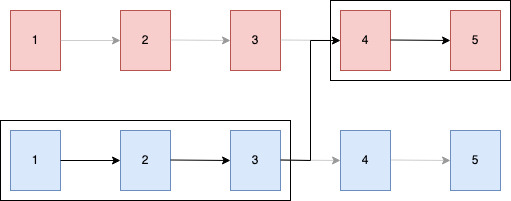
\includegraphics[width=12cm]{stitch.jpg}
      \caption*{This diagram gives us a simple view of a stitched network. The black arrows denote the flow of data, while
      the grey arrows denote the flow of data that would have been present, had the two networks been used without stitching.
      The different blocks denote different layers (numbered) and the different colors denote different neural networks. The arrow
      from layer 3 of the blue network to layer 4 of the red network involves a simple stitch transformation, though it is left
      out of the image for concision. The boxed layers, plus the stitch, make up the stitched network. In this specific case,
      the stitched network's task accuracy asks as our similarity measure for red layer 3 with 
      blue layer 3, since red layer 4 expects the input to come from red layer 3.}
   \end{figure}
\end{center}

\section{Experimental Setup}
\label{ExperimentalSetup}
\subsection*{Models and Dataset}
We use the CIFAR-10 dataset with small ResNets. We chose CIFAR-10 because it is a small, well-understood dataset
of small RGB-images that we can train fast on. We chose ResNets because they were used by Bansal et al., giving our
results more context.

We compare all different
layers of ResNet34 and all
ResNets with between 10 and 18 layers. These small ResNets we characterize with 4-tuples, where 
each element is either 1 or 2, representing the number of residual blocks per blockset\footnote{
   Residual blocks are partitioned into sets of consecutive within which they have the same shape.
} out of the 4 blocksets
present in a ResNet.\footnote{
   Though within each block there are two layers,
   we focus on stitching out of and into blocks for simplicity.
} Since we never use 10 or more blocks per blockset, we can denote these 4-tuples unambiguously\footnote{
   If we were to refer to them by their numbers of layers there would be ambiguity, since the neural networks
   r1122 and r2211 have the same number of layers, but different shapes per layer if we were to map their
   layers one to one.
} as
r1111, r1112, and so on. This set of 16 ResNets\footnote{
   Since each element of the 4-tuple is either 1 or 2, there are 16 total choices.
} we refer to as the small ResNets.

Our small ResNets' representations double in depth and half in both width and height every blockset
The first depth is 64 and the first width and height
are both 32. Because the input dimensions have a depth of 3, and a width and height both of 32, ResNets have an
initial convolutional layer before the first blockset. Because the output dimension is a 10-dimensional vector,
for classification, they also have a fully connected layer at the very end.

\subsection*{Experiment}
We train ResNet34 as well as each possible small resnet on CIFAR, yielding an accuracy above 90\%. Because 
there are 16 such possible
small ResNets and we stitch every possible ordered pair\footnote{
   For example, stitching r1111 with r2222.
}, there are around 256 such pairs we stitch amongst the small
ResNets. In addition, we stitch ResNet34 to ResNet18 and vice versa to see whether our findings generalize to a
bigger network. In every ordered pair of networks being stitched, the former is the sender, and the latter
is the receiver. For any sender/receiver pair, we stitch into all layers of the receiver
excluding both the convolution and any layers inside the residual blocks. We stitch out of all layers from the sender
excluding both the fully connected layer and any layers inside the residual blocks. 
Note that we do stitch out of and into all blocks per blockset if there is more than one.

We use randomly initialized ResNets as controls. Unlike Bansal et al., we only vary our neural networks by their
initialization weights. Otherwise our setup is nearly identical.
For every pair of networks that are stitched, we also create a random sender and a random
receiver both with the same architecture as the sender and receiver respectively. Just as the sender is stitched
into the receiver, the random sender is stitched into both the receiver and the random receiver, and the sender
is also stitched into the random receiver. This allows us to acertain that the stitches
are not overly powerful \cite{Bansal2021RevisitingMS}. The stitches are trained on
the standard CIFAR-10 classification task by using backpropagation through the stitched network.

We train each stitch for 4 epochs. This hyperparameter was selected after experimentation. For both
regular training of the network and training of the stitches we use stochastic gradient descent with momentum 0.9,
batch size 256, weight decay 0.01, learning rate 0.01, and a post-warmup cosine learning rate scheduler.
These hyperparameters were also arrived at from experimentation. The code will be available on Github.

For ordered pair of networks, we plot the accuracy of all the stitches between their prefixes and suffixes
on a grid based on the sending layer and the receiver layer. The layer is
denoted by an integer which counts how many layers came before it\footnote{
   The initial convolution is ``0,'' the first block of the first blockset is ``1,'' and so on.
}.

Because one of our goals is to see whether stitches emulate the receiver's expected representation, we
also measure the final pointwise mean squared difference between representations generated by stitch and
those that are expected. This mean squared difference is a crude numerical method, 
but gives us a sense of whether the representations
the stitch generates are close to the expected ones, since if they are close, the difference ought to be very close
to zero. We use random networks for to give us a sense what a high mean squared difference
looks like, numerically. Additionally, we use a ``similarity'' trained stitch to give us a sense of what a low mean
squared difference looks like. The similarity trained stitch is not trained using backpropagation
from the classification task, but instead on the mean squared loss corresponding to the mean squared difference.
It gives us a sense of what mean squared difference the stitch could reach if it truly were ``doing its best''
to emulate the expected representation. We found that we had to train these other stitches for around 30 epochs.

\section{Results}
\label{Results}
\subsection*{Preliminary Results}
All our experimental results are formatted as layer to
layer similarity matrices. (The row is the sender, the column is the receiver, and the compared layers are the expected sender
and the sender; the entry is the accuracy of the stitched network).

Every single pair in our experiment has the same
patterns. When two random networks are stitched, all possible stitches have low accuracy with a rather uniform distribution. When
a sender is stiched with a random receiver, only stitches from the later layers of the sender into the later layers of the (random)
receiver have high stitching accuracy. When a random sender is stitched into a receiver, only stitches into the early layers of the
receiver have high stitching accuracy. When the sender is stitched into the receiver, all layers in the lower left hand triangle
of the layer-to-layer similarity matrix have high stitching accuracy. 
This intruiging last result was most apparent for small ResNets or different shapes.
Figures are below for all our results.

For larger ResNets of the same shape we saw more of a diagonal pattern (akin to Bansal et al.) though, the lower left hand triangle for small
ResNets had higher
accuracy than the top right hand triangle by a lot. 
The cause for the triangle for smaller networks is mysterious. We believe that
it is possible that the stitch is not learning to emulate the expected representation but instead create another representation
that yields the same results (i.e. high accuracy). We are using a rough numerical estimate to understand this. Namely, we
are using the mean squared error between the expected representation and the representation produced by the stitched network.
We provide statistics and an analysis below. We also provide the results of a similarity-trained set of stitches which
try to copy the expected representation. These are meant mainly to give us a sense of how close a stitch could be to the
expected representation if it were ``trying'' to copy it. We find that these similarity-trained stitches are not very good
and perhaps not that similar from the corresponding normal (sometimes called ``vanilla'') stitch.

\label{Figure2}
\begin{center}
   \begin{figure}[h!]
      \centering
      \caption{Triangle Pattern in Small ResNets}
      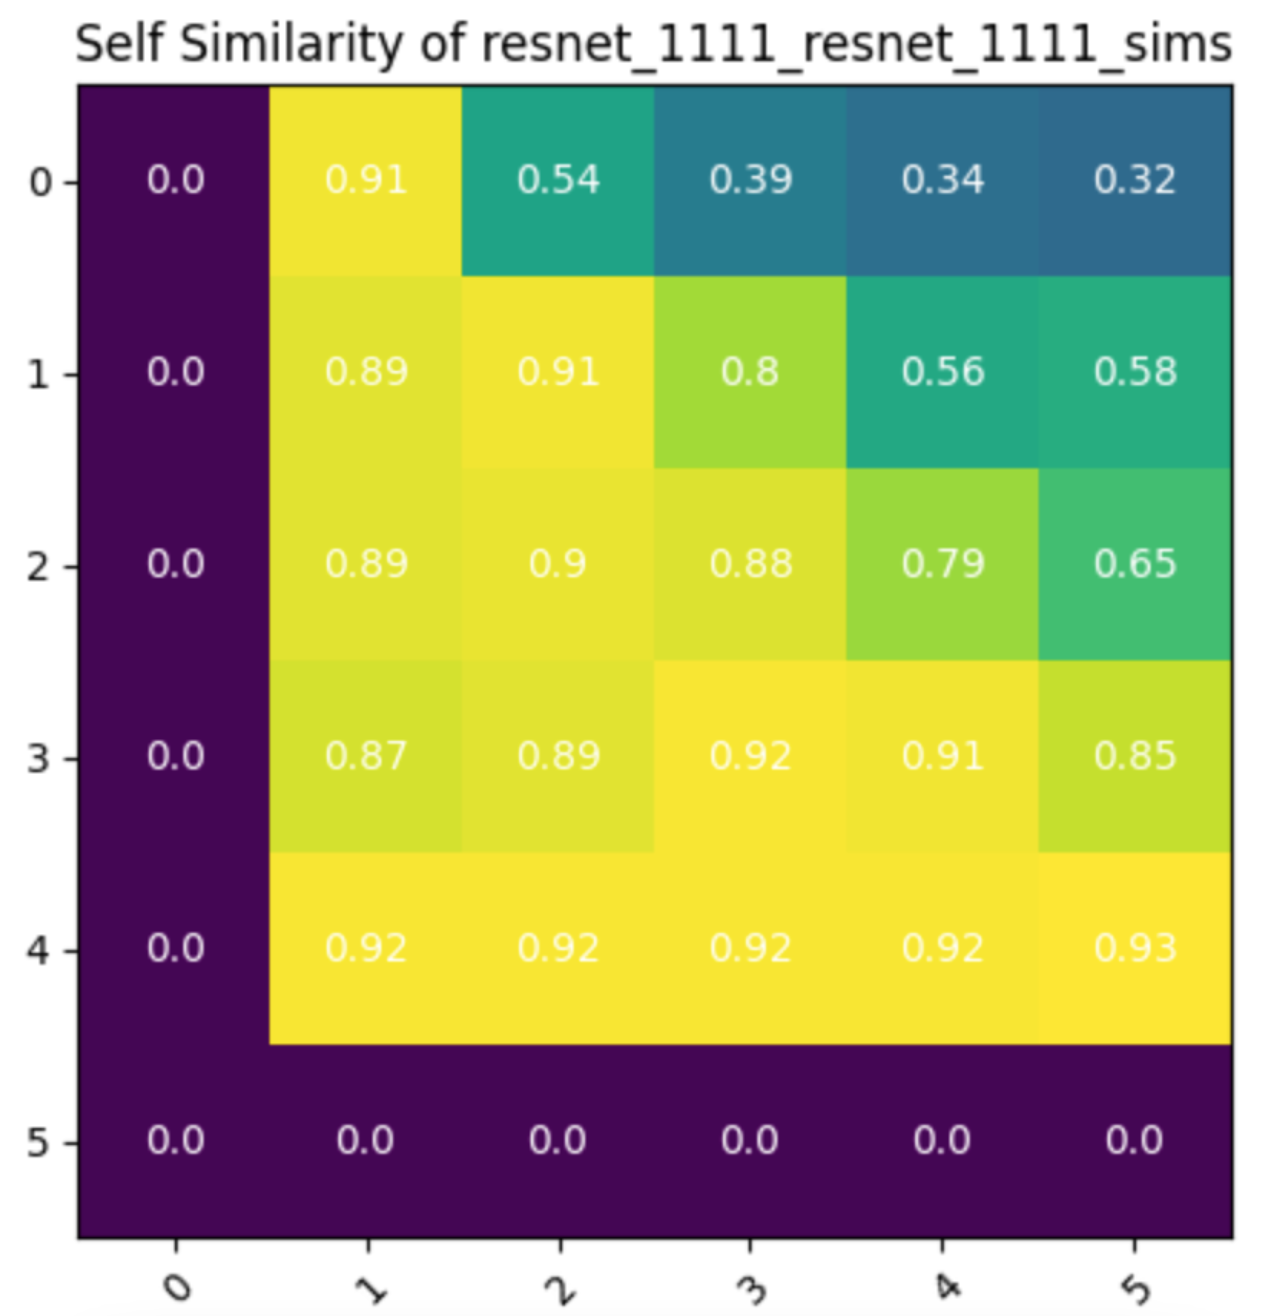
\includegraphics[width=6.5cm]{resnet1111_1111.png}
      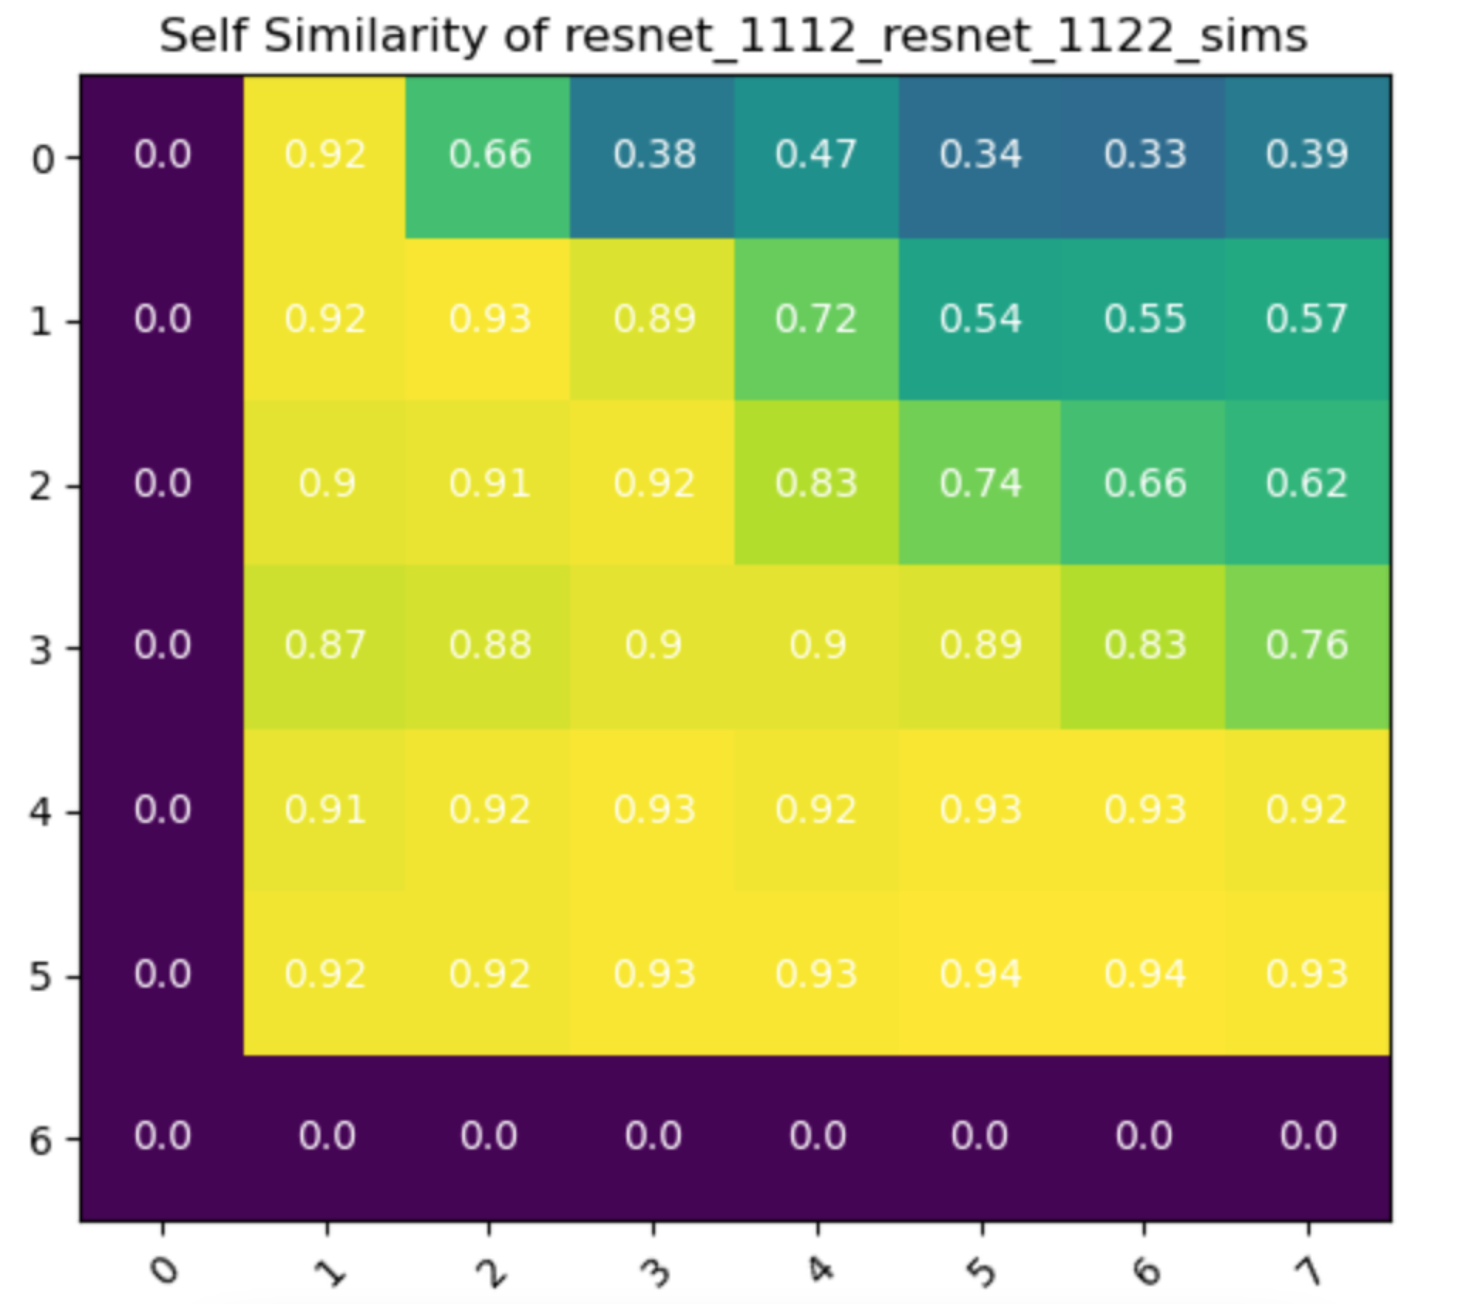
\includegraphics[width=6.5cm]{resnet1112_1122.png}
      \caption*{These are similarity matrices from sender to receiver. The row tells you the sending layer and the column tells you the recieving layer.
      The entry tells you the accuracy of the stitched model created by stitching between those two layers.}
   \end{figure}
\end{center}

\label{Figure3}
\begin{center}
   \begin{figure}[h!]
      \centering
      \caption{Sometimes a Diagonal in Large ResNets}
      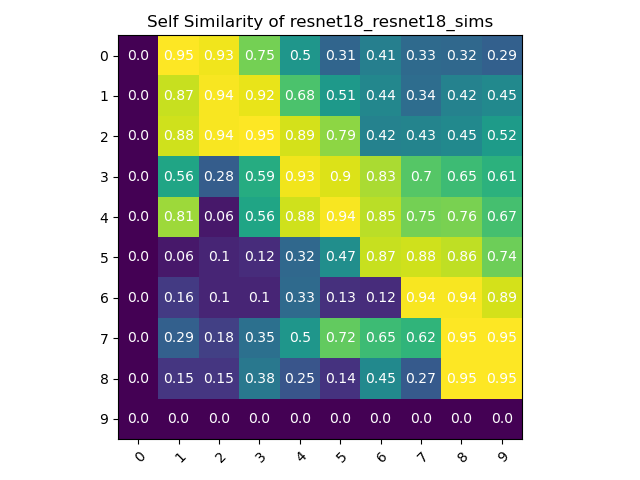
\includegraphics[width=8.5cm]{resnet18_resnet18_sims.png}
      \caption*{Similariy matrix from sender to receiver.}
   \end{figure}
\end{center}

\label{Figure4}
\begin{center}
   \begin{figure}[h!]
      \centering
      \caption{Sometimes Triangular Pattern in Large ResNets}
      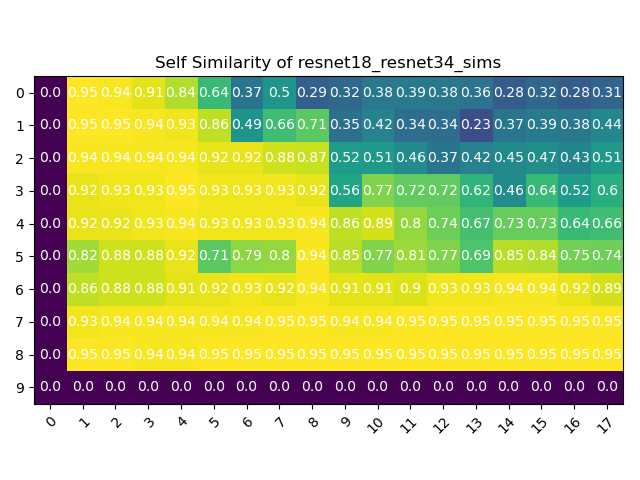
\includegraphics[width=9.5cm]{resnet18_resnet34_sims.png}
      \caption*{Similariy matrix from sender to receiver.}
   \end{figure}
\end{center}

\subsection*{Controls}
As previously mentioned we used random networks to control for stitching power. Nothing particularly interesting
came out of our controls. This was as we had hoped. A couple examples are below in figure 5. The main result from the controls
was that as the randomly initialized (untrained) fraction of the stitched network grew, the accuracy went down.

\label{Figure5}
\begin{center}
   \begin{figure}[h!]
      \centering
      \caption{Triangle Pattern in Small ResNets}
      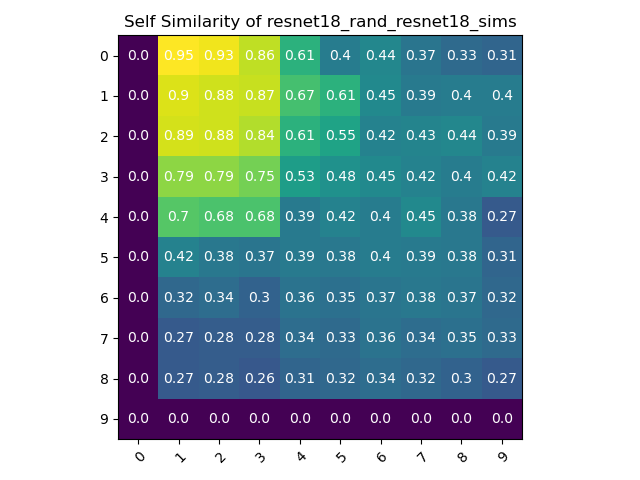
\includegraphics[width=8.5cm]{resnet18_rand_resnet18_sims.png}
      \caption*{Similarity matrix from random ResNet18 to trained ResNet18.}
   \end{figure}
\end{center}

\subsection*{Interpretation}
\subsubsection*{What We Had Expected}
The reason that these results are perplexing is that we were expecting to see some sort of diagonal in the similarity matrix
when stitching
different networks. Bansal et al.'s findings suggested that there would be a one-to-one layer correspondence between
two networks of the same architecture. While we did, roughly, see this for ResNet18 and ResNet34, we did not for the
small ResNets. Obviously, it is impossible to have a diagonal when the sender and receiver have different lengths,
but we had considered a few possibilities.

Namely, we considered that there may be a one-to-one correspondence between subsections of each neural network to
form some kind of ``strided diagonal''. In the layer one-to-one correspondence case, we interpret the correspondence
to tell us that the layers are learning the same representation. In the subsection one-to-one correspondence case
(the ``strided diagonal'') we interpret that to mean that there are black-box sections of each neural network which
have the same final learned representation.

To make our language more precise we can define consecutive sequences of neural networks as ``modules''. Naturally,
modules have modules within them and, if they are not the entirety of the network, they are within a module. We thought
that there would be some non-trivial modular mapping between two networks. That is to say, there would be some way of
describing the sender as a sequence of modules and the receiver as a sequence of modules, such that a mapping existed
between the two sequences. Obviously, the trivial mapping exists between the entire sender to the entire receiver
(since they both input identical images and both output nearly identical classifications), but we had hoped for more.

Implicit in our expectations, naturally, was the assumption that there would be a \textbf{mapping} between some quantity
in the sender and some other quantity in the receiver. It is highly unintuitive that layers in the sender are equally
similar (and very much so) to lots of layers in the receiver. We expected each layer to have at most one to three layers
in the other network it was similar to. As we've seen, however, later layers tend to be similar to nearly all earlier layers
by our stitching metric.

\subsection*{What This Might Mean}
We see two main explanations for the results: small ResNets on CIFAR-10 could be able to maintain most if not all of the image
information throughout their processing of the image and the stitches are learning to create representations which yield high
accuracy despite being different from their expected counterparts.

The former option is very interesting because it upheaves our understanding of neural networks. Normally we assume that
as data is more deeply processed in neural networks it becomes more ``high level'' and granular information is lost. If
this were not the case it would prompt us to understand when and why that is so. The latter option is compelling mainly
because it helps us find a limitation of stitching. In a sense it would mean that stitches are powerful enough to ``hack''
the receiver network: to trick it into using a representation it was not expecting. If this were possible and common, then
high stitching accuracy would not be a sign of similarity, though low stitching accuracy could be a sign of dissimilarity.

We mainly examine the latter option by using a similarity-trained stitch and by taking statistics on the mean squared
error (difference) of the stitches with respect to (mainly) the expected representation. A high mean squared error would
imply that the stitch is more likely to be different, while a low mean squared error would imply that the stitch is more
likely to be similar. It is a crude measurement, but we include it as a taste of what may be possible in the future. The
similariy trained stitch, on the other hand, is meant to give us a sense of how close a stitch could be to the expected
representation if that were it's only ``goal''. In both cases we use controls in the form of stitches with or between
random networks.

\subsection*{Similarity-Trained-Trained Stitch}
Below we have a heatmap of the task accuracy for the similarity-trained stitch. We found that it was not
easy to train a stitch exclusively using mean squared error with respect to the expected representation. We suspect
that there may be subspaces of the representation space that are far more relevant to accuracy and that by using
mean squared error the similarity-trained stitch has to try much, much harder to get any results (which it fails
to get here). For context, we only needed around 1 epoch to train regular, vanilla stitches to reach competitive accuracy
with the original network and around 4 to reach nearly identical accuracy. For the similarity-trained stitch, we used 30
epochs per stitch and have close to random accuracy.

\label{Figure6}
\begin{center}
   \begin{figure}[h!]
      \centering
      \caption{Naive Similarity-Trained Training Tends To Fail}
      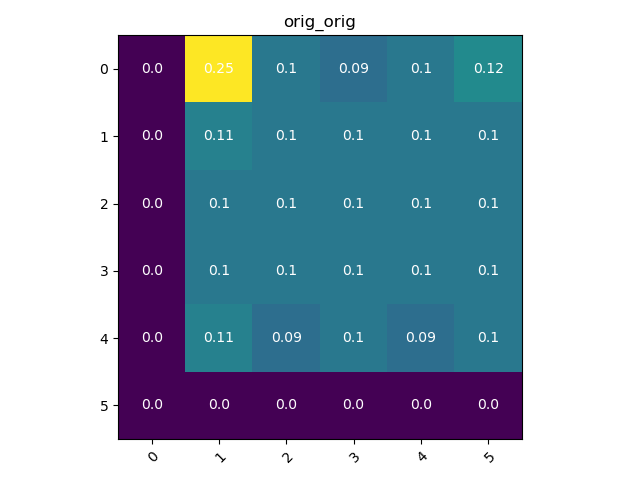
\includegraphics[width=7.5cm]{resnet1111_1111_autoencoder.png}
      \caption*{Similarity matrix from sender to receiver.}
   \end{figure}
\end{center}

\subsection*{Numerical Analysis}
We examined the diagonal of nine pairs of stitched networks: 2211 with 2211, 1211 with 1211, 
2121 with 2121, 2111 with 2111, 2221 with 2221, 1121 with 1121, 1112 with 1112, 1111 with 1111, 
and 1221 with 1221. We compared trained networks with random ones (and vice versa) as well as trained
networks with the same trained network and random networks amongst eachother.\footnote{NANs were encountered for 
Traineed to Random for both the autoencoder and vanilla stitches when comparing with the original on the diagonal.
This probably means  that there were
very large numbers which means that some distances were too long to be computed meaning implying that
the representations were totally, randomly, differnet. When we compared the entire tables, we got NANs and infinities
for various cases with random representations.}

That is to say, we measured the mean squared distance (frobenius norm) of the stitched representations for the networks
for each of those pairs of networks, specifically for the representations that were at the same layer. This enabled us
to get a sense for whether the networks were learning the same representation or ``hacking'' eachother.

We also computed the same statistics on the set of all stitches to see if the diagonal was any different. We focused
on the diagonal because due to Bansal et. al. we have more confidence in it corresponding to a true emulation of the
expected representation.

What we tended to find was that for random networks the mean squared distance was high and for trained networks it was
low. It tended to be around two orders of magnitude lower for the similarity-trained stitch, which is expected, but the
similarity trained stitch does not seem to be further from the expected representation than the vanilla stitch is from it
(in ``Similarity-Trained Stitches vs. Vanilla Stitches''). The specifics (tables) are in the appendix.
   
\section{Conclusion}
\label{Conclusion}
It appears that stitching does not behave for different architectures exactly as we had hoped, though it does not seem
to be generating representations altogether different from those that were expected. We hypothesize that in some cases
stitches may be able to ``hack'' the receiver by learning to give it novel representations which nonetheless yield high
accuracy. However, it appears that stitches do not deviate, numerically, that much from the expected representation on
average. Most likely, there are subspaces in the representation space more important than others and the vanilla stitch
is able to optimize them, potentially at the expense of others, thus yielding slightly higher mean squared error with
respect to the expected representation than is possible using a purely mean squared error trained stitch. We see this
by training such a stitch (the ``Similarity-Trained'' stitch). In line with this conclusion, the similarity stitch struggles
to reach high accuracy, probably because it is to ``diversified'' and does not have information about what subspaces
matter more for the downstream task.

\section*{Acknowledgments}
\label{Acknowledgments}
Thank you to the SuperUROP benefactors (MIT EECS) for funding this project as well as my mentors, and the
SuperUROP faculty and staff for helping me embark on this research and write this paper.
\newpage
\bibliography{iclr2021_conference}
\bibliographystyle{iclr2021_conference}
\newpage
\appendix
\section{Appendix}
\label{Appendix}
Below are numerical talbes for the mean squared differences between different representations
after training with different stitching methods. Vanilla stitches were trained using backpropagation
through the stitched network from the CIFAR-10 classification task. Similarity-Trained stitches were
trained using a mean squared error loss with respect to the expected representation of the
receiver layer.

We compile tables of simple statistics for the mean squared differences both for all the stitches as well
as for the diagonals, which we expect to tend to exhibit smaller mean squared differences. For each comparison
we use stitches to and from randomly weighted models as controls.

\subsection*{Diagonals: Vanilla Stitches}
\label{Table1}
\begin{tabular}{c c c c c}
   Model Pair&Minimum&Mean&Maximum&Standard Deviation\\
   Trained to Trained&2.03e-03&4.41e-02&2.80e-01&6.10e-02\\
   Trained to Random&1.27e-01&4.28e+05&4.24e+06&1.12e+06\\
   Random to Trained&1.50e-02&3.25e-01&5.29e-01&1.56e-01\\
   Random to Random&1.58e-01&1.26e+02&1.36e+03&2.92e+02\\
\end{tabular}

\label{Table2}
\subsection*{Diagonals: Similarity-Trained Stitches}
\begin{tabular}{c c c c c}
   Model Pair&Minimum&Mean&Maximum&Standard Deviation\\
   Trained to Trained&2.15e-05&1.50e-02&1.91e-01&3.73e-02\\
   Trained to Random&5.52e-02&7.60e+04&3.56e+05&1.26e+05\\
   Random to Trained&3.48e-05&1.10e-03&5.91e-03&2.01e-03\\
   Random to Random&1.73e-02&4.94e+00&6.03e+01&1.27e+01\\
\end{tabular}

\label{Table3}
\subsection*{Diagonals: Similarity-Trained Stitches vs. Vanilla Stitches}
\begin{tabular}{c c c c c}
   Model Pair&Minimum&Mean&Maximum&Standard Deviation\\
   Trained to Trained&1.21e-03&2.33e-02&1.14e-01&3.89e-02\\
   Trained to Random&2.71e-03&1.67e+05&3.67e+06&7.32e+05\\
   Random to Trained&7.94e-03&3.23e-01&5.29e-01&1.59e-01\\
   Random to Random&1.17e-01&1.18e+02&1.35e+03&2.86e+02\\
\end{tabular}

\label{Table4}
\subsection*{All Representation Pairs: Vanilla Stitches}
\begin{tabular}{c c c c c}
   Model Pair&Minimum&Mean&Maximum&Standard Deviation\\
   Trained to Trained&1.63e-03&4.49e-02&3.63e+00&1.37e-01\\
   Trained to Random&1.55e-04&2.63e+05&1.78e+07&1.00e+06\\
   Random to Trained&1.35e-02&2.21e+00&2.27e+02&1.17e+01\\
   Random to Random&1.34e-01&7.25e+04&1.24e+07&5.94e+05\\
\end{tabular}

\label{Table5}
\subsection*{All Representation Pairs: Similarity-Trained Stitches}
\begin{tabular}{c c c c c}
   Model Pair&Minimum&Mean&Maximum&Standard Deviation\\
   Trained to Trained&5.39e-06&1.58e-02&1.32e+00&5.90e-02\\
   Trained to Random&1.71e-07&1.06e+05&9.19e+06&4.27e+05\\
   Random to Trained&6.32e-06&2.05e-03&1.88e-02&4.31e-03\\
   Random to Random&1.59e-02&4.20e+04&6.90e+06&3.44e+05\\
\end{tabular}

\label{Table6}
\subsection*{All Representation Pairs: Similarity-Trained Stitches vs. Vanilla Stitches}
\begin{tabular}{c c c c c}
   Model Pair&Minimum&Mean&Maximum&Standard Deviation\\
   Trained to Trained&7.83e-04&1.98e-02&5.87e-01&3.25e-02\\
   Trained to Random&1.54e-04&6.26e+04&5.79e+06&3.43e+05\\
   Random to Trained&7.94e-03&2.21e+00&2.27e+02&1.17e+01\\
   Random to Random&9.44e-02&2.12e+04&4.77e+06&2.08e+05\\
\end{tabular}

\end{document}
